% Options for packages loaded elsewhere
% Options for packages loaded elsewhere
\PassOptionsToPackage{unicode}{hyperref}
\PassOptionsToPackage{hyphens}{url}
\PassOptionsToPackage{dvipsnames,svgnames,x11names}{xcolor}
%
\documentclass[
  letterpaper,
  DIV=11,
  numbers=noendperiod]{scrreprt}
\usepackage{xcolor}
\usepackage{amsmath,amssymb}
\setcounter{secnumdepth}{5}
\usepackage{iftex}
\ifPDFTeX
  \usepackage[T1]{fontenc}
  \usepackage[utf8]{inputenc}
  \usepackage{textcomp} % provide euro and other symbols
\else % if luatex or xetex
  \usepackage{unicode-math} % this also loads fontspec
  \defaultfontfeatures{Scale=MatchLowercase}
  \defaultfontfeatures[\rmfamily]{Ligatures=TeX,Scale=1}
\fi
\usepackage{lmodern}
\ifPDFTeX\else
  % xetex/luatex font selection
\fi
% Use upquote if available, for straight quotes in verbatim environments
\IfFileExists{upquote.sty}{\usepackage{upquote}}{}
\IfFileExists{microtype.sty}{% use microtype if available
  \usepackage[]{microtype}
  \UseMicrotypeSet[protrusion]{basicmath} % disable protrusion for tt fonts
}{}
\makeatletter
\@ifundefined{KOMAClassName}{% if non-KOMA class
  \IfFileExists{parskip.sty}{%
    \usepackage{parskip}
  }{% else
    \setlength{\parindent}{0pt}
    \setlength{\parskip}{6pt plus 2pt minus 1pt}}
}{% if KOMA class
  \KOMAoptions{parskip=half}}
\makeatother
% Make \paragraph and \subparagraph free-standing
\makeatletter
\ifx\paragraph\undefined\else
  \let\oldparagraph\paragraph
  \renewcommand{\paragraph}{
    \@ifstar
      \xxxParagraphStar
      \xxxParagraphNoStar
  }
  \newcommand{\xxxParagraphStar}[1]{\oldparagraph*{#1}\mbox{}}
  \newcommand{\xxxParagraphNoStar}[1]{\oldparagraph{#1}\mbox{}}
\fi
\ifx\subparagraph\undefined\else
  \let\oldsubparagraph\subparagraph
  \renewcommand{\subparagraph}{
    \@ifstar
      \xxxSubParagraphStar
      \xxxSubParagraphNoStar
  }
  \newcommand{\xxxSubParagraphStar}[1]{\oldsubparagraph*{#1}\mbox{}}
  \newcommand{\xxxSubParagraphNoStar}[1]{\oldsubparagraph{#1}\mbox{}}
\fi
\makeatother

\usepackage{color}
\usepackage{fancyvrb}
\newcommand{\VerbBar}{|}
\newcommand{\VERB}{\Verb[commandchars=\\\{\}]}
\DefineVerbatimEnvironment{Highlighting}{Verbatim}{commandchars=\\\{\}}
% Add ',fontsize=\small' for more characters per line
\usepackage{framed}
\definecolor{shadecolor}{RGB}{241,243,245}
\newenvironment{Shaded}{\begin{snugshade}}{\end{snugshade}}
\newcommand{\AlertTok}[1]{\textcolor[rgb]{0.68,0.00,0.00}{#1}}
\newcommand{\AnnotationTok}[1]{\textcolor[rgb]{0.37,0.37,0.37}{#1}}
\newcommand{\AttributeTok}[1]{\textcolor[rgb]{0.40,0.45,0.13}{#1}}
\newcommand{\BaseNTok}[1]{\textcolor[rgb]{0.68,0.00,0.00}{#1}}
\newcommand{\BuiltInTok}[1]{\textcolor[rgb]{0.00,0.23,0.31}{#1}}
\newcommand{\CharTok}[1]{\textcolor[rgb]{0.13,0.47,0.30}{#1}}
\newcommand{\CommentTok}[1]{\textcolor[rgb]{0.37,0.37,0.37}{#1}}
\newcommand{\CommentVarTok}[1]{\textcolor[rgb]{0.37,0.37,0.37}{\textit{#1}}}
\newcommand{\ConstantTok}[1]{\textcolor[rgb]{0.56,0.35,0.01}{#1}}
\newcommand{\ControlFlowTok}[1]{\textcolor[rgb]{0.00,0.23,0.31}{\textbf{#1}}}
\newcommand{\DataTypeTok}[1]{\textcolor[rgb]{0.68,0.00,0.00}{#1}}
\newcommand{\DecValTok}[1]{\textcolor[rgb]{0.68,0.00,0.00}{#1}}
\newcommand{\DocumentationTok}[1]{\textcolor[rgb]{0.37,0.37,0.37}{\textit{#1}}}
\newcommand{\ErrorTok}[1]{\textcolor[rgb]{0.68,0.00,0.00}{#1}}
\newcommand{\ExtensionTok}[1]{\textcolor[rgb]{0.00,0.23,0.31}{#1}}
\newcommand{\FloatTok}[1]{\textcolor[rgb]{0.68,0.00,0.00}{#1}}
\newcommand{\FunctionTok}[1]{\textcolor[rgb]{0.28,0.35,0.67}{#1}}
\newcommand{\ImportTok}[1]{\textcolor[rgb]{0.00,0.46,0.62}{#1}}
\newcommand{\InformationTok}[1]{\textcolor[rgb]{0.37,0.37,0.37}{#1}}
\newcommand{\KeywordTok}[1]{\textcolor[rgb]{0.00,0.23,0.31}{\textbf{#1}}}
\newcommand{\NormalTok}[1]{\textcolor[rgb]{0.00,0.23,0.31}{#1}}
\newcommand{\OperatorTok}[1]{\textcolor[rgb]{0.37,0.37,0.37}{#1}}
\newcommand{\OtherTok}[1]{\textcolor[rgb]{0.00,0.23,0.31}{#1}}
\newcommand{\PreprocessorTok}[1]{\textcolor[rgb]{0.68,0.00,0.00}{#1}}
\newcommand{\RegionMarkerTok}[1]{\textcolor[rgb]{0.00,0.23,0.31}{#1}}
\newcommand{\SpecialCharTok}[1]{\textcolor[rgb]{0.37,0.37,0.37}{#1}}
\newcommand{\SpecialStringTok}[1]{\textcolor[rgb]{0.13,0.47,0.30}{#1}}
\newcommand{\StringTok}[1]{\textcolor[rgb]{0.13,0.47,0.30}{#1}}
\newcommand{\VariableTok}[1]{\textcolor[rgb]{0.07,0.07,0.07}{#1}}
\newcommand{\VerbatimStringTok}[1]{\textcolor[rgb]{0.13,0.47,0.30}{#1}}
\newcommand{\WarningTok}[1]{\textcolor[rgb]{0.37,0.37,0.37}{\textit{#1}}}

\usepackage{longtable,booktabs,array}
\usepackage{calc} % for calculating minipage widths
% Correct order of tables after \paragraph or \subparagraph
\usepackage{etoolbox}
\makeatletter
\patchcmd\longtable{\par}{\if@noskipsec\mbox{}\fi\par}{}{}
\makeatother
% Allow footnotes in longtable head/foot
\IfFileExists{footnotehyper.sty}{\usepackage{footnotehyper}}{\usepackage{footnote}}
\makesavenoteenv{longtable}
\usepackage{graphicx}
\makeatletter
\newsavebox\pandoc@box
\newcommand*\pandocbounded[1]{% scales image to fit in text height/width
  \sbox\pandoc@box{#1}%
  \Gscale@div\@tempa{\textheight}{\dimexpr\ht\pandoc@box+\dp\pandoc@box\relax}%
  \Gscale@div\@tempb{\linewidth}{\wd\pandoc@box}%
  \ifdim\@tempb\p@<\@tempa\p@\let\@tempa\@tempb\fi% select the smaller of both
  \ifdim\@tempa\p@<\p@\scalebox{\@tempa}{\usebox\pandoc@box}%
  \else\usebox{\pandoc@box}%
  \fi%
}
% Set default figure placement to htbp
\def\fps@figure{htbp}
\makeatother





\setlength{\emergencystretch}{3em} % prevent overfull lines

\providecommand{\tightlist}{%
  \setlength{\itemsep}{0pt}\setlength{\parskip}{0pt}}



 


\KOMAoption{captions}{tableheading}
\makeatletter
\@ifpackageloaded{bookmark}{}{\usepackage{bookmark}}
\makeatother
\makeatletter
\@ifpackageloaded{caption}{}{\usepackage{caption}}
\AtBeginDocument{%
\ifdefined\contentsname
  \renewcommand*\contentsname{Table of contents}
\else
  \newcommand\contentsname{Table of contents}
\fi
\ifdefined\listfigurename
  \renewcommand*\listfigurename{List of Figures}
\else
  \newcommand\listfigurename{List of Figures}
\fi
\ifdefined\listtablename
  \renewcommand*\listtablename{List of Tables}
\else
  \newcommand\listtablename{List of Tables}
\fi
\ifdefined\figurename
  \renewcommand*\figurename{Figure}
\else
  \newcommand\figurename{Figure}
\fi
\ifdefined\tablename
  \renewcommand*\tablename{Table}
\else
  \newcommand\tablename{Table}
\fi
}
\@ifpackageloaded{float}{}{\usepackage{float}}
\floatstyle{ruled}
\@ifundefined{c@chapter}{\newfloat{codelisting}{h}{lop}}{\newfloat{codelisting}{h}{lop}[chapter]}
\floatname{codelisting}{Listing}
\newcommand*\listoflistings{\listof{codelisting}{List of Listings}}
\makeatother
\makeatletter
\makeatother
\makeatletter
\@ifpackageloaded{caption}{}{\usepackage{caption}}
\@ifpackageloaded{subcaption}{}{\usepackage{subcaption}}
\makeatother
\usepackage{bookmark}
\IfFileExists{xurl.sty}{\usepackage{xurl}}{} % add URL line breaks if available
\urlstyle{same}
\hypersetup{
  pdftitle={Mi Tesis},
  pdfauthor={Tu Nombre},
  colorlinks=true,
  linkcolor={blue},
  filecolor={Maroon},
  citecolor={Blue},
  urlcolor={Blue},
  pdfcreator={LaTeX via pandoc}}


\title{Mi Tesis}
\author{Tu Nombre}
\date{2025-06-17}
\begin{document}
\maketitle

\renewcommand*\contentsname{Table of contents}
{
\hypersetup{linkcolor=}
\setcounter{tocdepth}{2}
\tableofcontents
}

\bookmarksetup{startatroot}

\chapter{thesis}\label{thesis}

\section{Quarto}\label{quarto}

Quarto enables you to weave together content and executable code into a
finished document. To learn more about Quarto see
\url{https://quarto.org}.

\bookmarksetup{startatroot}

\chapter{}\label{section}

\bookmarksetup{startatroot}

\chapter{}\label{section-1}

\part{Estudio de caso}

\section*{Adaptación de PageRank a redes territoriales del estado de
Chiapas: Un enfoque basado en cadenas de
Markov}\label{adaptaciuxf3n-de-pagerank-a-redes-territoriales-del-estado-de-chiapas-un-enfoque-basado-en-cadenas-de-markov}
\addcontentsline{toc}{section}{Adaptación de PageRank a redes
territoriales del estado de Chiapas: Un enfoque basado en cadenas de
Markov}

\markright{Adaptación de PageRank a redes territoriales del estado de
Chiapas: Un enfoque basado en cadenas de Markov}

En situaciones de emergencia, como desastres naturales o crisis
humanitarias, es fundamental contar con mecanismos eficientes para
distribuir ayuda y recursos a la población afectada. En regiones como el
estado de Chiapas que cuenta con 124 municipios según el INEGI, contando
con una geografía montañosa y la dispersión de los municipios dificultan
la conectividad, se vuelve especialmente importante identificar puntos
estratégicos dentro de la red territorial que puedan facilitar la
logística y la respuesta rápida.

Para abordar este desafío, se propone aplicar el algoritmo PageRank,
desarrollado por Larry Page y Sergey Brin como parte del motor de
búsqueda de Google, con el fin de priorizar municipios según su
importancia dentro de la red de transporte intermunicipal. Este
algoritmo, basado en un modelo de cadenas de Markov, mide la relevancia
de cada nodo (municipio) al simular el recorrido de un ``navegante
aleatorio'' que transita la red con cierta probabilidad de seguir
conexiones o saltar aleatoriamente a otro nodo.

En términos prácticos, PageRank estima la probabilidad estacionaria de
una cadena de Markov con un número finito de estados describiendo la
fracción de tiempo que, en promedio, el sistema permanece en cada estado
cuando se observa durante un periodo suficientemente largo (REFERENCIA),
lo cual permite identificar aquellos municipios que, por su posición
estratégica y conectividad, tienen mayor influencia dentro del sistema
territorial. Esta información es clave para diseñar estrategias de
distribución de ayuda, optimización de rutas y toma de decisiones en
situaciones críticas.

En este estudio de caso, se aplica PageRank a la red territorial del
estado de Chiapas, representando los municipios como nodos y las rutas
entre ellos como enlaces ponderados por distancia. El objetivo es
obtener una clasificación de los municipios más centrales o influyentes,
que puedan actuar como puntos clave en escenarios de distribución
logística.

\section*{Problemas en la red y solución de
PageRank}\label{problemas-en-la-red-y-soluciuxf3n-de-pagerank}
\addcontentsline{toc}{section}{Problemas en la red y solución de
PageRank}

\markright{Problemas en la red y solución de PageRank}

En el análisis de una red de nodos, existen dos factores que pueden
obstaculizar la convergencia hacia una distribución estacionaria, estos
factores son: - los nodos colgantes - subgrafos ansorbentes

\subsection*{Nodos colgantes}\label{nodos-colgantes}
\addcontentsline{toc}{subsection}{Nodos colgantes}

Los nodos colgantes hace referencia a las páginas que no tiene enlaes de
salida. En el contexto de una red territorial, este fenómeno se
manifiesta en municipios que no tienen conexión con otros municipios. En
el caso del estado de Chiapas, no se identificaron nodos colgantes en la
red analizada.

El algoritmo PageRank soluciona este problema modificando la matriz de
red. Sea \(N\) la matriz de red (REFERENCIA), donde cada entrada
\(n_{ij}\) representa la conexión desde el nodo \(j\) hacia el nodo
\(i\), donde \(i,j \in \mathbb{N}\). Para abordar el problema de nodos
colgantes, se redefine la matriz de transición \(Q\) donde la entrada
\(i\) que tiene entradas cero (nodos colgantes) se remplaza por
\(\frac{1}{k}\) donde \(k\) es número totales de páginas o municipios,
esta corrección nos garantiza que la matriz de trancisión \(Q\) sea
estocástica.

\subsection*{Subgrafos absorbentes}\label{subgrafos-absorbentes}
\addcontentsline{toc}{subsection}{Subgrafos absorbentes}

Cuando existen subgrafos absorbentes dentro de la red. Estos
corresponden a conjuntos de páginas (o nodos) que están interconectados
entre sí pero no tienen enlaces de salida hacia el resto de la red, es
decir, hacen un ciclo. En el contexto de la red territorial, esto se
representa en los municipios que únicamente estan conectados entres sí,
formando un subconjunto cerrado que puede atrapar al navegante en un
ciclo sin posibilidad de salir.

Para resolver este problema, los creadores del algoritmo PageRank
introdujeron un mecanismo llamado factor de amortiguación. Este consiste
en asumir de la red una probabilidad \(1-p\) de teletranspotarse
aleatoriamente a cualquier otro nodo del grafo.

Usualmente se toma \(p=0.85\), esto significa que en un \(85\%\) de los
casos el navegante sigue los enklaces y el \(15\%\) restante salta
aleatoriamente a cualquier otro nodo.

Con los ajustes mencionados se obtene una matriz de trasción modificada
que se define como: \[P:= p Q +(1-p)A\] donde, \(A\) es una matriz
cuadrada con todas las entradas \(\dfrac{1}{k}\) representando una
conexión aleatoria uniforme. La matriz resultante \(P\) garantiza que el
algoritmo funcione correctamente y siempre llegue a una solución
estable, debido a que al ser estocástica, asegura que desde cada nodo
siempre conserve la probabilidad total en cada pso del proceso; al ser
aperiódica, evita que el sistema quede atrapado en ciclos repetitivos; y
al ser irreducible, garantiza que todos los nodos estén conectados de
alguna forma, permitiendo que eventualmente se pueda llegar a cualquier
parte de la red.

\chapter{Metodología}\label{metodologuxeda}

En esta sección se describe

\section{Recolección de datos}\label{recolecciuxf3n-de-datos}

El estudio utilizó dos fuentes principales de datos geoespaciales:

\begin{enumerate}
\def\labelenumi{\arabic{enumi}.}
\tightlist
\item
  \textbf{Datos de rutas}:

  \begin{itemize}
  \tightlist
  \item
    Obtenidos mediante la API de \href{http://project-osrm.org/}{Open
    Source Routing Machine} (OSRM).
  \item
    El formato usado son Coordenadas geográficas en WGS84
    (\texttt{{[}latitud,\ longitud{]}}) para cada punto de la ruta.
  \end{itemize}
\item
  \textbf{Datos de elevación}:

  \begin{itemize}
  \tightlist
  \item
    La información utilizada proviene del Modelo Digital de Elevación
    (DEM) generado por la misión Shuttle Radar Topography Mission (SRTM)
    de la NASA, disponible en NASA Earthdata
    (https://earthdata.nasa.gov/). Los datos cuentan con una resolución
    espacial de 30 metros y se distribuyen en teselas de
    \(1^{\circ} \times 1^{\circ}\) de latitud y longitud. Cada archivo
    ráster SRTM está conformado por una malla regular de celdas
    (pixeles), en la cual cada celda almacena un valor de elevación del
    terreno expresado en metros sobre el nivel del mar (m s. n.~m.).
    Para cubrir áreas de mayor extensión, como un estado, un país o una
    región montañosa, es necesario integrar estas teselas, lo que
    permite generar una capa continua y sin discontinuidades del
    relieve, denominada \textbf{mosaico ráster}.
  \end{itemize}
\end{enumerate}

\section{``Cálculo de distancia 3D de rutas geográficas usando datos
OSRM y
elevación''}\label{cuxe1lculo-de-distancia-3d-de-rutas-geogruxe1ficas-usando-datos-osrm-y-elevaciuxf3n}

Para estimar la longitud real de una carretera considerando las
variaciones de altitud del terreno, se utiliza una formulación basada en
la distancia geodésica entre puntos sucesivos de una ruta, combinada con
la diferencia de elevaciones. Esto permite obtener una distancia
tridimensional (3D) más realista, que considera tanto la curvatura
terrestre como los cambios topográficos.

Sea una ruta discretizada por \(N\) puntos geográficos con coordenadas:
\(P_i= (\phi_i, \lambda_i\)) para \(i=1, \cdots, N\) donde: \(\phi_i\)
es la latitud de punto \(i\) y \(\lambda_i\) es la longitud del punto
\(i\). ~ La distancia superficial (2D) entre dos puntos consecutivos se
calcula utilizando la fórmula de Vincenty o usando elipsoide WGS84
(World Geodetic System 1984), el cual se calcula mediante la siguiente
expresión ~\[
 d_i^{2D}:= GeodInv(\phi_{i-1}, \lambda_{i-1}, \phi_i, \lambda_i),
 \]

que representa la distancia geodésica 2D entre los puntos \(P_{i-1}\) y
\(P_{i},\) calculada sobre la superficie de la Tierra.

Por otro lado, para estimar la distancia real de una carretera,
considerando las variaciones del terreno (con elevación), se considera
la ruta como una secuencia de puntos geográficos
\(P_i= (\phi_i, \lambda_i\)) y \(h_i\) la elevación en metros sobre el
nivel del mar del punto \(i,\) extraÍda del mosaico ráster de altitudes
mediente la interpolacion espacial. La distancia entre dos puntos
consecutivos se calcula como \[
d_i^{3D} := \sqrt{(d_i^{2D})^2+(\Delta h_i)^2},
\] siendo \(\Delta h_i= h_i-h_{i-1}\) el cambio de altitud entre dos
puntos consecutivos.

La distancia total proyectada (2D) y la distancia real sobre el terreno
(3D) son respectivamente \[
D^{(2D)}:= \sum_{i=1}^{N-1} d_i^{(2D)},
\] y \[
D^{(3D)}:= \sum_{i=1}^{N-1} d_i^{(3D)}.
\]

\begin{Shaded}
\begin{Highlighting}[]
\ImportTok{from}\NormalTok{ google.colab }\ImportTok{import}\NormalTok{ drive}
\ImportTok{import}\NormalTok{ requests}
\ImportTok{import}\NormalTok{ csv}
\ImportTok{import}\NormalTok{ time}
\ImportTok{from}\NormalTok{ urllib.parse }\ImportTok{import}\NormalTok{ quote}
\ImportTok{import}\NormalTok{ folium}
\ImportTok{import}\NormalTok{ math}
\ImportTok{import}\NormalTok{ rasterio}
\ImportTok{from}\NormalTok{ rasterio.merge }\ImportTok{import}\NormalTok{ merge}
\ImportTok{from}\NormalTok{ shapely.geometry }\ImportTok{import}\NormalTok{ LineString}
\ImportTok{import}\NormalTok{ numpy }\ImportTok{as}\NormalTok{ np}
\ImportTok{from}\NormalTok{ pyproj }\ImportTok{import}\NormalTok{ Geod}
\ImportTok{import}\NormalTok{ matplotlib.pyplot }\ImportTok{as}\NormalTok{ plt}
\ImportTok{import}\NormalTok{ pandas }\ImportTok{as}\NormalTok{ pd}
\ImportTok{from}\NormalTok{ IPython.display }\ImportTok{import}\NormalTok{ display}

\CommentTok{\# Montar Google Drive}
\NormalTok{drive.mount(}\StringTok{\textquotesingle{}/content/drive\textquotesingle{}}\NormalTok{)}

\CommentTok{\# Instalar librerías necesarias}
\OperatorTok{!}\NormalTok{pip install rasterio geopandas pyproj folium}

\CommentTok{\# Configuración de ciudades}
\NormalTok{ciudades }\OperatorTok{=}\NormalTok{ [}
    \StringTok{"Acacoyagua"}\NormalTok{, }\StringTok{"Acala"}\NormalTok{, }\StringTok{"Acapetahua"}\NormalTok{, }\StringTok{"Aldama"}\NormalTok{, }\StringTok{"Altamirano"}\NormalTok{, }\StringTok{"Amatán"}\NormalTok{, }
    \StringTok{"Amatenango de la Frontera"}\NormalTok{, }\StringTok{"Amatenango del Valle"}\NormalTok{, }\StringTok{"Ángel Albino Corzo"}\NormalTok{,}
    \StringTok{"Arriaga"}\NormalTok{, }\StringTok{"Bejucal de Ocampo"}\NormalTok{, }\StringTok{"Bella Vista"}\NormalTok{, }
    \StringTok{"Benemérito de las Américas"}\NormalTok{,}\StringTok{"Berriozábal"}\NormalTok{, }\StringTok{"Bochil"}\NormalTok{, }\StringTok{"Cacahoatán"}\NormalTok{, }
    \StringTok{"Capitán Luis Ángel Vidal"}\NormalTok{, }\StringTok{"Catazajá"}\NormalTok{, }\StringTok{"Chalchihuitán"}\NormalTok{, }\StringTok{"Chamula"}\NormalTok{, }
    \StringTok{"Chanal"}\NormalTok{, }\StringTok{"Chapultenango"}\NormalTok{,}\StringTok{"Chenalhó"}\NormalTok{, }\StringTok{"Chiapa de Corzo"}\NormalTok{, }\StringTok{"Chiapilla"}\NormalTok{, }
    \StringTok{"Chicoasén"}\NormalTok{, }\StringTok{"Chicomuselo"}\NormalTok{, }\StringTok{"Chilón"}\NormalTok{,}\StringTok{"Cintalapa de Figueroa"}\NormalTok{, }\StringTok{"Coapilla"}\NormalTok{, }
    \StringTok{"Comitán de Domínguez"}\NormalTok{, }\StringTok{"Copainalá"}\NormalTok{, }\StringTok{"El Bosque"}\NormalTok{, }\StringTok{"El Parral"}\NormalTok{,}
    \StringTok{"El Porvenir"}\NormalTok{, }\StringTok{"Emiliano Zapata"}\NormalTok{, }\StringTok{"Escuintla"}\NormalTok{, }\StringTok{"Francisco León"}\NormalTok{, }
    \StringTok{"Frontera Comalapa"}\NormalTok{, }\StringTok{"Frontera Hidalgo"}\NormalTok{, }\StringTok{"Honduras de la Sierra"}\NormalTok{,}
    \StringTok{"Huehuetán"}\NormalTok{, }\StringTok{"Huitiupán"}\NormalTok{, }\StringTok{"Huixtán"}\NormalTok{, }\StringTok{"Huixtla"}\NormalTok{, }\StringTok{"Ixhuatán"}\NormalTok{,}
    \StringTok{"Ixtacomitán"}\NormalTok{, }\StringTok{"Ixtapa"}\NormalTok{, }\StringTok{"Ixtapangajoya"}\NormalTok{, }\StringTok{"Jiquipilas"}\NormalTok{, }\StringTok{"Jitotol"}\NormalTok{, }
    \StringTok{"Juárez"}\NormalTok{, }\StringTok{"La Concordia"}\NormalTok{, }\StringTok{"La Grandeza"}\NormalTok{, }\StringTok{"La Independencia"}\NormalTok{, }
    \StringTok{"La Libertad"}\NormalTok{, }\StringTok{"La Trinitaria"}\NormalTok{, }\StringTok{"Larráinzar"}\NormalTok{, }\StringTok{"Las Margaritas"}\NormalTok{, }
    \StringTok{"Las Rosas"}\NormalTok{, }\StringTok{"Mapastepec"}\NormalTok{, }\StringTok{"Maravilla Tenejapa"}\NormalTok{, }\StringTok{"Marqués de Comillas"}\NormalTok{,}
    \StringTok{"Mazapa de Madero"}\NormalTok{, }\StringTok{"Mazatán"}\NormalTok{, }\StringTok{"Metapa"}\NormalTok{, }\StringTok{"Mezcalapa"}  \StringTok{"Mitontic"}\NormalTok{, }
    \StringTok{"Montecristo de Guerrero"}\NormalTok{, }\StringTok{"Motozintla"}\NormalTok{, }\StringTok{"Nicolás Ruíz"}\NormalTok{, }\StringTok{"Ocosingo"}\NormalTok{, }
    \StringTok{"Ocotepec"}\NormalTok{, }\StringTok{"Ocozocoautla de Espinosa"}\NormalTok{, }\StringTok{"Ostuacán"}\NormalTok{, }\StringTok{"Osumacinta"}\NormalTok{, }
    \StringTok{"Oxchuc"}\NormalTok{, }\StringTok{"Palenque"}\NormalTok{, }\StringTok{"Pantelhó"}\NormalTok{, }\StringTok{"Pantepec"}\NormalTok{, }\StringTok{"Pichucalco"}\NormalTok{,}
    \StringTok{"Pijijiapan"}\NormalTok{, }\StringTok{"Pueblo Nuevo Solistahuacán"}\NormalTok{, }\StringTok{"Rayón"}\NormalTok{, }\StringTok{"Reforma"}\NormalTok{, }
    \StringTok{"Rincón Chamula San Pedro"}\NormalTok{, }\StringTok{"Sabanilla"}\NormalTok{, }\StringTok{"Salto de Agua"}\NormalTok{, }
    \StringTok{"San Andrés Duraznal"}\NormalTok{, }\StringTok{"San Cristóbal de las Casas"}\NormalTok{, }\StringTok{"San Fernando"}\NormalTok{, }
    \StringTok{"San Juan Cancuc"}\NormalTok{, }\StringTok{"San Lucas"}\NormalTok{, }\StringTok{"Santiago el Pinar"}\NormalTok{, }\StringTok{"Siltepec"}\NormalTok{, }
    \StringTok{"Simojovel"}\NormalTok{, }\StringTok{"Sitalá"}\NormalTok{, }\StringTok{"Socoltenango"}\NormalTok{, }\StringTok{"Solosuchiapa"}\NormalTok{, }\StringTok{"Soyaló"}\NormalTok{, }
    \StringTok{"Suchiapa"}\NormalTok{, }\StringTok{"Suchiate"}\NormalTok{, }\StringTok{"Sunuapa"}\NormalTok{, }\StringTok{"Tapachula"}\NormalTok{, }\StringTok{"Tapalapa"}\NormalTok{, }\StringTok{"Tapilula"}\NormalTok{,}
    \StringTok{"Tecpatán"}\NormalTok{, }\StringTok{"Tenejapa"}\NormalTok{, }\StringTok{"Teopisca"}\NormalTok{, }\StringTok{"Tila"}\NormalTok{, }\StringTok{"Tonalá"}\NormalTok{, }\StringTok{"Totolapa"}\NormalTok{,}
    \StringTok{"Tumbalá"}\NormalTok{, }\StringTok{"Tuxtla Chico"}\NormalTok{, }\StringTok{"Tuxtla Gutiérrez"}\NormalTok{, }\StringTok{"Tuzantán"}\NormalTok{, }\StringTok{"Tzimol"}\NormalTok{, }
    \StringTok{"Unión Juárez"}\NormalTok{, }\StringTok{"Venustiano Carranza"}\NormalTok{,  }\StringTok{"Villa Comaltitlán"}\NormalTok{, }
    \StringTok{"Villa Corzo"}\NormalTok{, }\StringTok{"Villaflores"}\NormalTok{, }\StringTok{"Yajalón"}\NormalTok{, }\StringTok{"Zinacantán"}
\NormalTok{]}
\NormalTok{ciudades.sort()}

\CommentTok{\# Funciones auxiliares}
\KeywordTok{def}\NormalTok{ cargar\_mosaico\_srtm():}
\NormalTok{    archivos\_hgt }\OperatorTok{=}\NormalTok{ [}
        \StringTok{"/content/drive/MyDrive/thesis/chiapas\_hgt/N17W094.hgt"}\NormalTok{,}
        \StringTok{"/content/drive/MyDrive/thesis/chiapas\_hgt/N17W093.hgt"}\NormalTok{,}
        \StringTok{"/content/drive/MyDrive/thesis/chiapas\_hgt/N17W092.hgt"}\NormalTok{,}
        \StringTok{"/content/drive/MyDrive/thesis/chiapas\_hgt/N16W095.hgt"}\NormalTok{,}
        \StringTok{"/content/drive/MyDrive/thesis/chiapas\_hgt/N16W094.hgt"}\NormalTok{,}
        \StringTok{"/content/drive/MyDrive/thesis/chiapas\_hgt/N16W093.hgt"}\NormalTok{,}
        \StringTok{"/content/drive/MyDrive/thesis/chiapas\_hgt/N15W094.hgt"}\NormalTok{,}
        \StringTok{"/content/drive/MyDrive/thesis/chiapas\_hgt/N15W092.hgt"}\NormalTok{,}
        \StringTok{"/content/drive/MyDrive/thesis/chiapas\_hgt/N14W093.hgt"}\NormalTok{,}
        \StringTok{"/content/drive/MyDrive/thesis/chiapas\_hgt/N16W091.hgt"}\NormalTok{,}
        \StringTok{"/content/drive/MyDrive/thesis/chiapas\_hgt/N15W093.hgt"}\NormalTok{,}
        \StringTok{"/content/drive/MyDrive/thesis/chiapas\_hgt/N16W092.hgt"}
\NormalTok{    ]}
\NormalTok{    src\_files }\OperatorTok{=}\NormalTok{ [rasterio.}\BuiltInTok{open}\NormalTok{(f) }\ControlFlowTok{for}\NormalTok{ f }\KeywordTok{in}\NormalTok{ archivos\_hgt]}
\NormalTok{    mosaico, transform }\OperatorTok{=}\NormalTok{ merge(src\_files)}
    \ControlFlowTok{for}\NormalTok{ src }\KeywordTok{in}\NormalTok{ src\_files:}
\NormalTok{        src.close()}
    \ControlFlowTok{return}\NormalTok{ mosaico, transform}

\KeywordTok{def}\NormalTok{ obtener\_coordenadas(ciudad):}
\NormalTok{    url }\OperatorTok{=} \SpecialStringTok{f"https://nominatim.openstreetmap.org/search?q=}
\ErrorTok{        \{quote}\NormalTok{(ciudad}\OperatorTok{+}\StringTok{\textquotesingle{}, Chiapas, México\textquotesingle{}}\NormalTok{)\}}\OperatorTok{\&}\BuiltInTok{format}\OperatorTok{=}\NormalTok{json}\StringTok{"}
\ErrorTok{    response = requests.get}\NormalTok{(url, headers}\OperatorTok{=}\NormalTok{\{}\StringTok{\textquotesingle{}User{-}Agent\textquotesingle{}}\NormalTok{: }\StringTok{\textquotesingle{}Mozilla/5.0\textquotesingle{}}\NormalTok{\})}
\NormalTok{    data }\OperatorTok{=}\NormalTok{ response.json()}
    \ControlFlowTok{if}\NormalTok{ data:}
        \ControlFlowTok{return}\NormalTok{ (}\BuiltInTok{float}\NormalTok{(data[}\DecValTok{0}\NormalTok{][}\StringTok{\textquotesingle{}lat\textquotesingle{}}\NormalTok{]), }\BuiltInTok{float}\NormalTok{(data[}\DecValTok{0}\NormalTok{][}\StringTok{\textquotesingle{}lon\textquotesingle{}}\NormalTok{]))}
    \ControlFlowTok{return} \VariableTok{None}

\KeywordTok{def}\NormalTok{ obtener\_ruta\_osrm(coord\_origen, coord\_destino):}
\NormalTok{    lon1, lat1 }\OperatorTok{=}\NormalTok{ coord\_origen[}\DecValTok{1}\NormalTok{], coord\_origen[}\DecValTok{0}\NormalTok{]}
\NormalTok{    lon2, lat2 }\OperatorTok{=}\NormalTok{ coord\_destino[}\DecValTok{1}\NormalTok{], coord\_destino[}\DecValTok{0}\NormalTok{]}
\NormalTok{    url }\OperatorTok{=} \SpecialStringTok{f"http://router.project{-}osrm.org/route/v1/driving/}\SpecialCharTok{\{}\NormalTok{lon1}\SpecialCharTok{\}}\SpecialStringTok{,}\SpecialCharTok{\{}\NormalTok{lat1}\SpecialCharTok{\}}\SpecialStringTok{;}
\ErrorTok{        \{lon2\},\{lat2\}?overview=full\&geometries=geojson"}
    \ControlFlowTok{try}\NormalTok{:}
\NormalTok{        response }\OperatorTok{=}\NormalTok{ requests.get(url)}
\NormalTok{        data }\OperatorTok{=}\NormalTok{ response.json()}
        \ControlFlowTok{if}\NormalTok{ data[}\StringTok{\textquotesingle{}code\textquotesingle{}}\NormalTok{] }\OperatorTok{==} \StringTok{\textquotesingle{}Ok\textquotesingle{}}\NormalTok{:}
\NormalTok{            distancia }\OperatorTok{=}\NormalTok{ data[}\StringTok{\textquotesingle{}routes\textquotesingle{}}\NormalTok{][}\DecValTok{0}\NormalTok{][}\StringTok{\textquotesingle{}distance\textquotesingle{}}\NormalTok{]}
\NormalTok{            duracion }\OperatorTok{=}\NormalTok{ data[}\StringTok{\textquotesingle{}routes\textquotesingle{}}\NormalTok{][}\DecValTok{0}\NormalTok{][}\StringTok{\textquotesingle{}duration\textquotesingle{}}\NormalTok{]}
\NormalTok{            geometria }\OperatorTok{=}\NormalTok{ data[}\StringTok{\textquotesingle{}routes\textquotesingle{}}\NormalTok{][}\DecValTok{0}\NormalTok{][}\StringTok{\textquotesingle{}geometry\textquotesingle{}}\NormalTok{][}\StringTok{\textquotesingle{}coordinates\textquotesingle{}}\NormalTok{]}
            \ControlFlowTok{return}\NormalTok{ distancia, duracion, [(lat, lon) }\ControlFlowTok{for}\NormalTok{ lon, lat }\KeywordTok{in}\NormalTok{ geometria]}
    \ControlFlowTok{except} \PreprocessorTok{Exception} \ImportTok{as}\NormalTok{ e:}
        \BuiltInTok{print}\NormalTok{(}\SpecialStringTok{f"Error OSRM: }\SpecialCharTok{\{}\NormalTok{e}\SpecialCharTok{\}}\SpecialStringTok{"}\NormalTok{)}
    \ControlFlowTok{return} \VariableTok{None}\NormalTok{, }\VariableTok{None}\NormalTok{, }\VariableTok{None}

\KeywordTok{def}\NormalTok{ calcular\_distancia\_3d\_ruta(mosaico, transform, ruta\_coords):}
\NormalTok{    geod }\OperatorTok{=}\NormalTok{ Geod(ellps}\OperatorTok{=}\StringTok{"WGS84"}\NormalTok{)}
\NormalTok{    distancia\_3d }\OperatorTok{=} \DecValTok{0}
\NormalTok{    distancia\_2d }\OperatorTok{=} \DecValTok{0}
\NormalTok{    elevaciones }\OperatorTok{=}\NormalTok{ []}
    \ControlFlowTok{for}\NormalTok{ coord }\KeywordTok{in}\NormalTok{ ruta\_coords:}
\NormalTok{        lon, lat }\OperatorTok{=}\NormalTok{ coord[}\DecValTok{1}\NormalTok{], coord[}\DecValTok{0}\NormalTok{]}
        \ControlFlowTok{try}\NormalTok{:}
\NormalTok{            col, row }\OperatorTok{=} \OperatorTok{\textasciitilde{}}\NormalTok{transform }\OperatorTok{*}\NormalTok{ (lon, lat)}
\NormalTok{            elev }\OperatorTok{=}\NormalTok{ mosaico[}\DecValTok{0}\NormalTok{, }\BuiltInTok{int}\NormalTok{(row), }\BuiltInTok{int}\NormalTok{(col)]}
\NormalTok{            elevaciones.append(elev)}
        \ControlFlowTok{except}\NormalTok{:}
\NormalTok{            elevaciones.append(np.nan)}
    \ControlFlowTok{for}\NormalTok{ i }\KeywordTok{in} \BuiltInTok{range}\NormalTok{(}\DecValTok{1}\NormalTok{, }\BuiltInTok{len}\NormalTok{(ruta\_coords)):}
\NormalTok{        lon1, lat1 }\OperatorTok{=}\NormalTok{ ruta\_coords[i}\OperatorTok{{-}}\DecValTok{1}\NormalTok{][}\DecValTok{1}\NormalTok{], ruta\_coords[i}\OperatorTok{{-}}\DecValTok{1}\NormalTok{][}\DecValTok{0}\NormalTok{]}
\NormalTok{        lon2, lat2 }\OperatorTok{=}\NormalTok{ ruta\_coords[i][}\DecValTok{1}\NormalTok{], ruta\_coords[i][}\DecValTok{0}\NormalTok{]}
\NormalTok{        elev1, elev2 }\OperatorTok{=}\NormalTok{ elevaciones[i}\OperatorTok{{-}}\DecValTok{1}\NormalTok{], elevaciones[i]}
        \ControlFlowTok{if}\NormalTok{ np.isnan(elev1) }\KeywordTok{or}\NormalTok{ np.isnan(elev2):}
            \ControlFlowTok{continue}
\NormalTok{        \_, \_, dist2d }\OperatorTok{=}\NormalTok{ geod.inv(lon1, lat1, lon2, lat2)}
\NormalTok{        delta\_elev }\OperatorTok{=}\NormalTok{ elev2 }\OperatorTok{{-}}\NormalTok{ elev1}
\NormalTok{        dist3d }\OperatorTok{=}\NormalTok{ math.sqrt(}\BuiltInTok{abs}\NormalTok{(dist2d}\OperatorTok{**}\DecValTok{2} \OperatorTok{+}\NormalTok{ delta\_elev}\OperatorTok{**}\DecValTok{2}\NormalTok{)) }
\NormalTok{        distancia\_2d }\OperatorTok{+=}\NormalTok{ dist2d}
\NormalTok{        distancia\_3d }\OperatorTok{+=}\NormalTok{ dist3d}
    \ControlFlowTok{return}\NormalTok{ distancia\_2d, distancia\_3d, elevaciones}

\CommentTok{\# Proceso principal}
\NormalTok{mosaico, transform }\OperatorTok{=}\NormalTok{ cargar\_mosaico\_srtm()}
\NormalTok{coordenadas }\OperatorTok{=}\NormalTok{ \{\}}
\BuiltInTok{print}\NormalTok{(}\StringTok{"Obteniendo coordenadas..."}\NormalTok{)}
\ControlFlowTok{for}\NormalTok{ ciudad }\KeywordTok{in}\NormalTok{ ciudades:}
\NormalTok{    coord }\OperatorTok{=}\NormalTok{ obtener\_coordenadas(ciudad)}
    \ControlFlowTok{if}\NormalTok{ coord:}
\NormalTok{        coordenadas[ciudad] }\OperatorTok{=}\NormalTok{ coord}
        \BuiltInTok{print}\NormalTok{(}\SpecialStringTok{f"}\SpecialCharTok{\{}\NormalTok{ciudad}\SpecialCharTok{\}}\SpecialStringTok{: }\SpecialCharTok{\{}\NormalTok{coord[}\DecValTok{0}\NormalTok{]}\SpecialCharTok{:.4f\}}\SpecialStringTok{, }\SpecialCharTok{\{}\NormalTok{coord[}\DecValTok{1}\NormalTok{]}\SpecialCharTok{:.4f\}}\SpecialStringTok{"}\NormalTok{)}
\NormalTok{    time.sleep(}\DecValTok{1}\NormalTok{)}

\NormalTok{archivo\_salida }\OperatorTok{=}
    \CommentTok{"/content/drive/MyDrive/thesis/ponencia\_pagerank\_distancia\_chiapas}
\ErrorTok{    /distancias\_chiapas\_carreteras\_3d\_completo.csv"}
\ControlFlowTok{with} \BuiltInTok{open}\NormalTok{(archivo\_salida, }\StringTok{"w"}\NormalTok{, newline}\OperatorTok{=}\StringTok{""}\NormalTok{, }
\NormalTok{    encoding}\OperatorTok{=}\StringTok{"utf{-}8"}\NormalTok{) }\ImportTok{as} \BuiltInTok{file}\NormalTok{:}
\NormalTok{    writer }\OperatorTok{=}\NormalTok{ csv.writer(}\BuiltInTok{file}\NormalTok{)}
\NormalTok{    writer.writerow([}\StringTok{"Origen"}\NormalTok{, }\StringTok{"Destino"}\NormalTok{, }\StringTok{"Distancia carretera (km)"}\NormalTok{, }
        \StringTok{"Distancia 3D (km)"}\NormalTok{, }\StringTok{"Diferencia (km)"}\NormalTok{, }\StringTok{"Tiempo estimado (min)"}\NormalTok{])}

\NormalTok{    mapa }\OperatorTok{=}\NormalTok{ folium.Map(location}\OperatorTok{=}\NormalTok{[}\FloatTok{16.75}\NormalTok{, }\OperatorTok{{-}}\FloatTok{92.62}\NormalTok{], zoom\_start}\OperatorTok{=}\DecValTok{8}\NormalTok{)}
\NormalTok{    colores }\OperatorTok{=}\NormalTok{ [}\StringTok{\textquotesingle{}red\textquotesingle{}}\NormalTok{, }\StringTok{\textquotesingle{}blue\textquotesingle{}}\NormalTok{, }\StringTok{\textquotesingle{}green\textquotesingle{}}\NormalTok{, }\StringTok{\textquotesingle{}purple\textquotesingle{}}\NormalTok{, }\StringTok{\textquotesingle{}orange\textquotesingle{}}\NormalTok{, }\StringTok{\textquotesingle{}darkred\textquotesingle{}}\NormalTok{]}

    \ControlFlowTok{for}\NormalTok{ i }\KeywordTok{in} \BuiltInTok{range}\NormalTok{(}\BuiltInTok{len}\NormalTok{(ciudades)):}
        \ControlFlowTok{for}\NormalTok{ j }\KeywordTok{in} \BuiltInTok{range}\NormalTok{(}\BuiltInTok{len}\NormalTok{(ciudades)):}
            \ControlFlowTok{if}\NormalTok{ i }\OperatorTok{==}\NormalTok{ j:}
                \ControlFlowTok{continue}
\NormalTok{            origen }\OperatorTok{=}\NormalTok{ ciudades[i]}
\NormalTok{            destino }\OperatorTok{=}\NormalTok{ ciudades[j]}
            \ControlFlowTok{if}\NormalTok{ origen }\KeywordTok{in}\NormalTok{ coordenadas }\KeywordTok{and}\NormalTok{ destino }\KeywordTok{in}\NormalTok{ coordenadas:}
                \BuiltInTok{print}\NormalTok{(}\SpecialStringTok{f"}\CharTok{\textbackslash{}n}\SpecialStringTok{Calculando }\SpecialCharTok{\{}\NormalTok{origen}\SpecialCharTok{\}}\SpecialStringTok{ → }\SpecialCharTok{\{}\NormalTok{destino}\SpecialCharTok{\}}\SpecialStringTok{..."}\NormalTok{)}
\NormalTok{                coord\_origen }\OperatorTok{=}\NormalTok{ coordenadas[origen]}
\NormalTok{                coord\_destino }\OperatorTok{=}\NormalTok{ coordenadas[destino]}
\NormalTok{                distancia\_ruta, duracion, ruta\_coords }\OperatorTok{=} 
\NormalTok{                    obtener\_ruta\_osrm(coord\_origen, coord\_destino)}
                \ControlFlowTok{if}\NormalTok{ ruta\_coords:}
\NormalTok{                    dist2d, dist3d, elevaciones }\OperatorTok{=}
\NormalTok{                        calcular\_distancia\_3d\_ruta(mosaico, transform,}
\NormalTok{                             ruta\_coords)}
                    \ControlFlowTok{if}\NormalTok{ dist2d }\OperatorTok{\textgreater{}} \DecValTok{0} \KeywordTok{and}\NormalTok{ dist3d }\OperatorTok{\textgreater{}} \DecValTok{0}\NormalTok{:}
\NormalTok{                        dist\_ruta\_km }\OperatorTok{=}\NormalTok{ distancia\_ruta}\OperatorTok{/}\DecValTok{1000}
\NormalTok{                        dist3d\_km }\OperatorTok{=}\NormalTok{ dist3d}\OperatorTok{/}\DecValTok{1000}
\NormalTok{                        diferencia }\OperatorTok{=}\NormalTok{ dist3d\_km }\OperatorTok{{-}}\NormalTok{ dist\_ruta\_km}
\NormalTok{                        tiempo\_min }\OperatorTok{=}\NormalTok{ duracion}\OperatorTok{/}\DecValTok{60}
\NormalTok{                        writer.writerow([origen, destino,}
                            \BuiltInTok{round}\NormalTok{(dist\_ruta\_km, }\DecValTok{3}\NormalTok{), }\BuiltInTok{round}\NormalTok{(dist3d\_km, }\DecValTok{3}\NormalTok{),}
                            \BuiltInTok{round}\NormalTok{(diferencia, }\DecValTok{3}\NormalTok{), }\BuiltInTok{round}\NormalTok{(tiempo\_min, }\DecValTok{1}\NormalTok{)])}
\NormalTok{                        color }\OperatorTok{=}\NormalTok{ colores[(i}\OperatorTok{+}\NormalTok{j) }\OperatorTok{\%} \BuiltInTok{len}\NormalTok{(colores)]}
\NormalTok{                        folium.PolyLine(locations}\OperatorTok{=}\NormalTok{ruta\_coords, color}\OperatorTok{=}\NormalTok{color,}
\NormalTok{                                        weight}\OperatorTok{=}\DecValTok{3}\NormalTok{, opacity}\OperatorTok{=}\FloatTok{0.7}\NormalTok{,tooltip}\OperatorTok{=}
                                        \SpecialStringTok{f"}\SpecialCharTok{\{}\NormalTok{origen}\SpecialCharTok{\}}\SpecialStringTok{ → }\SpecialCharTok{\{}\NormalTok{destino}\SpecialCharTok{\}}\SpecialStringTok{\textless{}br\textgreater{}Distancia:}
\ErrorTok{                                        \{dist\_ruta\_km:.1f\}km\textless{}br\textgreater{}Tiempo:}
\NormalTok{                                        \{tiempo\_min:}\FloatTok{.1}\ErrorTok{f}\NormalTok{\}min}\StringTok{").add\_to(mapa)}
\ErrorTok{                        folium.Marker}\NormalTok{(location}\OperatorTok{=}\NormalTok{coord\_origen, popup}\OperatorTok{=}\NormalTok{origen, }
\NormalTok{                            icon}\OperatorTok{=}\NormalTok{folium.Icon(color}\OperatorTok{=}\StringTok{\textquotesingle{}green\textquotesingle{}}\NormalTok{)).add\_to(mapa)}
\NormalTok{                        folium.Marker(location}\OperatorTok{=}\NormalTok{coord\_destino, popup}\OperatorTok{=}\NormalTok{destino, }
\NormalTok{                            icon}\OperatorTok{=}\NormalTok{folium.Icon(color}\OperatorTok{=}\StringTok{\textquotesingle{}red\textquotesingle{}}\NormalTok{)).add\_to(mapa)}
\NormalTok{                time.sleep(}\DecValTok{1}\NormalTok{)}

\BuiltInTok{print}\NormalTok{(}\SpecialStringTok{f"}\CharTok{\textbackslash{}n}\SpecialStringTok{ Datos guardados en }\SpecialCharTok{\{}\NormalTok{archivo\_salida}\SpecialCharTok{\}}\SpecialStringTok{"}\NormalTok{)}
\BuiltInTok{print}\NormalTok{(}\StringTok{" Mapa actualizado con rutas en ambas direcciones"}\NormalTok{)}

\CommentTok{\# Mostrar mapa directamente en Colab}
\NormalTok{display(mapa)}

\CommentTok{\# Mostrar CSV resultante}
\NormalTok{df }\OperatorTok{=}\NormalTok{ pd.read\_csv(archivo\_salida)}
\NormalTok{display(df)}
\end{Highlighting}
\end{Shaded}

\bookmarksetup{startatroot}

\chapter{}\label{section-2}

\bookmarksetup{startatroot}

\chapter{Mapa con Folium}\label{mapa-con-folium}

\bookmarksetup{startatroot}

\chapter{Mapa interactivo con Folium}\label{mapa-interactivo-con-folium}

\begin{Shaded}
\begin{Highlighting}[]
\ImportTok{import}\NormalTok{ folium}

\CommentTok{\# Crear el mapa centrado en Tuxtla Gutiérrez}
\NormalTok{mapa }\OperatorTok{=}\NormalTok{ folium.Map(location}\OperatorTok{=}\NormalTok{[}\FloatTok{16.7529}\NormalTok{, }\OperatorTok{{-}}\FloatTok{93.1169}\NormalTok{], zoom\_start}\OperatorTok{=}\DecValTok{13}\NormalTok{)}

\CommentTok{\# Agregar un marcador}
\NormalTok{folium.Marker(}
\NormalTok{    [}\FloatTok{16.7529}\NormalTok{, }\OperatorTok{{-}}\FloatTok{93.1169}\NormalTok{],}
\NormalTok{    tooltip}\OperatorTok{=}\StringTok{"Tuxtla Gutiérrez"}\NormalTok{,}
\NormalTok{    popup}\OperatorTok{=}\StringTok{"Capital de Chiapas"}
\NormalTok{).add\_to(mapa)}

\CommentTok{\# Guardar el mapa como archivo HTML para Selenium}
\NormalTok{mapa.save(}\StringTok{"mapa\_folium.html"}\NormalTok{)}
\end{Highlighting}
\end{Shaded}

\begin{Shaded}
\begin{Highlighting}[]
\ImportTok{import}\NormalTok{ IPython}
\NormalTok{IPython.display.display(mapa)}
\end{Highlighting}
\end{Shaded}

\begin{verbatim}
<folium.folium.Map at 0x292d0536510>
\end{verbatim}

\begin{Shaded}
\begin{Highlighting}[]
\CommentTok{\# Captura del mapa como imagen PNG para incluir en PDF}
\CommentTok{\# Captura del mapa como imagen PNG para incluir en PDF}
\ImportTok{import}\NormalTok{ os}
\ImportTok{from}\NormalTok{ selenium }\ImportTok{import}\NormalTok{ webdriver}
\ImportTok{from}\NormalTok{ selenium.webdriver.chrome.options }\ImportTok{import}\NormalTok{ Options}
\ImportTok{from}\NormalTok{ PIL }\ImportTok{import}\NormalTok{ Image}
\ImportTok{import}\NormalTok{ time}

\ControlFlowTok{if} \KeywordTok{not}\NormalTok{ os.path.exists(}\StringTok{"mapa\_folium.png"}\NormalTok{):}
\NormalTok{    options }\OperatorTok{=}\NormalTok{ Options()}
\NormalTok{    options.add\_argument(}\StringTok{\textquotesingle{}{-}{-}headless\textquotesingle{}}\NormalTok{)}
\NormalTok{    options.add\_argument(}\StringTok{\textquotesingle{}{-}{-}disable{-}gpu\textquotesingle{}}\NormalTok{)}
\NormalTok{    options.add\_argument(}\StringTok{\textquotesingle{}{-}{-}disable{-}dev{-}shm{-}usage\textquotesingle{}}\NormalTok{)}
\NormalTok{    options.add\_argument(}\StringTok{"{-}{-}window{-}size=800,600"}\NormalTok{)}

\NormalTok{    driver }\OperatorTok{=}\NormalTok{ webdriver.Chrome(options}\OperatorTok{=}\NormalTok{options)}

\NormalTok{    driver.get(}\StringTok{"file://"} \OperatorTok{+}\NormalTok{ os.path.abspath(}\StringTok{"mapa\_folium.html"}\NormalTok{))}
\NormalTok{    time.sleep(}\DecValTok{2}\NormalTok{)  }\CommentTok{\# Esperar a que cargue el mapa}

    \CommentTok{\# Forzar fondo blanco (evita fondo negro)}
\NormalTok{    driver.execute\_script(}\StringTok{"document.body.style.background = \textquotesingle{}white\textquotesingle{};"}\NormalTok{)}

    \CommentTok{\# Intentar capturar el contenedor del mapa directamente}
    \ControlFlowTok{try}\NormalTok{:}
\NormalTok{        map\_element }\OperatorTok{=}\NormalTok{ driver.find\_element(}\StringTok{"id"}\NormalTok{, }\StringTok{"map"}\NormalTok{)}
\NormalTok{        map\_element.screenshot(}\StringTok{"mapa\_folium.png"}\NormalTok{)}
    \ControlFlowTok{except}\NormalTok{:}
        \CommentTok{\# Si no encuentra el ID, captura toda la pantalla y recorta}
\NormalTok{        driver.save\_screenshot(}\StringTok{"mapa\_folium\_full.png"}\NormalTok{)}
\NormalTok{        img }\OperatorTok{=}\NormalTok{ Image.}\BuiltInTok{open}\NormalTok{(}\StringTok{"mapa\_folium\_full.png"}\NormalTok{)}
\NormalTok{        crop }\OperatorTok{=}\NormalTok{ img.crop((}\DecValTok{0}\NormalTok{, }\DecValTok{0}\NormalTok{, }\DecValTok{800}\NormalTok{, }\DecValTok{600}\NormalTok{))}
\NormalTok{        crop.save(}\StringTok{"mapa\_folium.png"}\NormalTok{)}

\NormalTok{    driver.quit()}
\end{Highlighting}
\end{Shaded}

\begin{figure}[H]

{\centering \pandocbounded{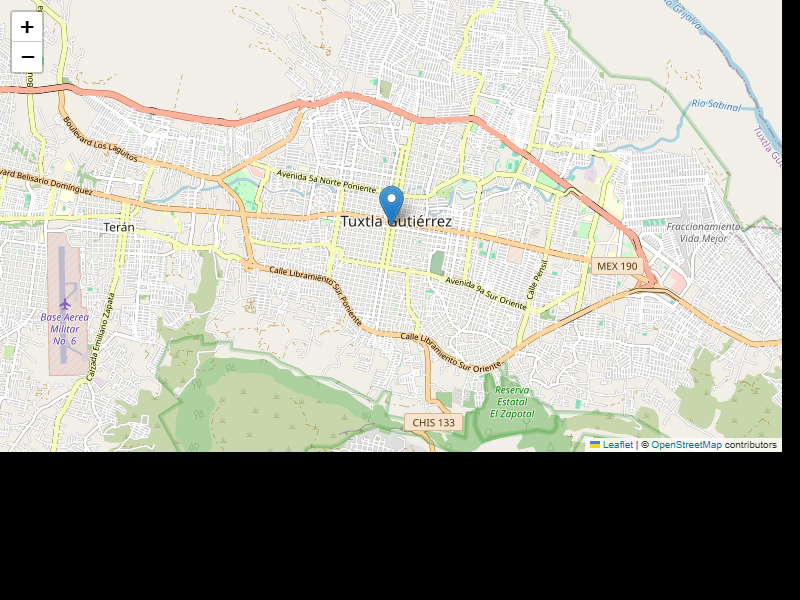
\includegraphics[keepaspectratio]{mapa_folium.png}}

}

\caption{Mapa generado con Folium}

\end{figure}%




\end{document}
